\chapter{Vorgehen}
\label{ch_vorgehen} 
Das Ziel ist die Entwicklung eines Prototypen aus dem bestehenden Modell der Projektarbeit von \cite{PA_bicycle}. Die Vorgehensschritte sind in der untenstehenden Auflistung abgebildet. Sie bilden die Struktur dieses Kapitels. Die Definition der konkreten Schritte geschah in Absprache mit Prof. Dr. M. Meli und dem Resarch Assitenten Herr Dario Dünar vom Instiut of Embedded Systems (InES). Auf der CD finden sich die Sitzungsprotokolle über den aktuellen Entwicklungsstand, die offenen Fragen und die Entscheidungen.

\subsubsection*{Liste der Arbeitschritte}
\label{liste} 

\begin{enumerate}
  \item Inbetriebnahme Machbarkeitsstudie  
  \item Hardware entwickeln  
  \item Inbetriebnahme Prototyp      
  \item Energy und Power Management
  \item Entwickeln einer BLE-Applikation       
 \end{enumerate}  

Die sprachliche Unterscheidung von Energy - und Power Management entspricht der Unterscheidung zweier \glqq Management-Teilen\grqq im Prototypen: Das Endprodukt regelt an zwei Stellen auf unterschiedliche Art die zur Verfügung stehende Energie. Der Begriff Energy Management wird in dieser Arbeit für das Sammeln und Weiterleiten von Energie über eine Hardwareimplementation gebraucht. Der Begriff Power Management wird für die Softwareimplementation gebraucht. Diese regelt, dass die zur Verfügung gestellte Energie nicht sofort verbraucht wird. Die sprachliche Trennung ist künstlich, denn in der Umsetzung spielen Hard- und Softwareregelung Hand in Hand. Die sprachliche Unterscheidung dient der Lesbarkeit und bezeichnet keinen physikalischen Unterschied.
 
 
 % 1---------------------------------------------------------------------------
 %------------------------------------------------------------------------------
  
 
\section{Inbetriebnahme Machbarkeitsstudie}\label{v_inbetriebnahme} 

      
Ziel der Inbetriebnahme des Aufbaus der vorangehenden Arbeit \cite{PA_bicycle} ist es, zu definieren, welche Funktionalitäten verbessert werden sollen. Zur Orientierung werden im ersten Unterkapitel \ref{fb} die Funktionsblöcke und deren Aufgaben festgehalten. Danach wird das Verhalten der Vorgängermodells in Unterkapitel \ref{verhalten} ausgemessen. Aus der Analyse entsteht die in Unterkapitel \ref{optimierung} aufgelistete erste Optimierungsliste. Als letztes folgt eine Vertiefung in das auffällige Verhalten des Eingangssignals in Unterkapitel \ref{auffaellig}. Dieser Exkurs hat Ursache in der Begegnung mit  Ives Théoduloz von EM MicroElectronic. Er entwickelte den in dieser Arbeit verwendete EM8500-Chip mit und wies uns auf den auffälligen Signalverlauf des Harvester-Eingangssignals (siehe Abbildung \ref{spannungMachbarkeit}) hin. Dieses Signal wurde deshalb bei der Inbetriebnahme eigens getestet, was im letzten Unterkapitel dokumentiert ist.
      
\subsection{Funktionsblöcke}\label{fb} 

Der Bicycle Computer besteht aus vier Funktionsblöcken, die in der Abbildung \ref{funktionsdiagramm_bild} dargestellt sind. Der erste Funktionsblock ist der Harvester (siehe 1) in der Abbildung \ref{funktionsdiagramm_bild}). Die Aufgaben des Harvesters ist es Energie zu Ernten und dem nächsten Funktionsblock ( Nummer 2) in der Abbildung  \ref{funktionsdiagramm_bild} zur Verfügung zu stellen. Der zweite Funktionsblock wird als Energy Management-Teil in der Arbeit bezeichnet. Die Aufgabe des zweiten Blocks ist es, Energie zu Sammeln und kontrolliert an die Verbrauchsstelle freizuschalten. Detaillierte Informationen finden sich in den Theoretischen Grundlagen im Unterkapitel \ref{t_energy_management}. Der dritte Funktionsblock ist der Ort, an dem die Energie verbraucht wird. In dieser Arbeit dient die Energie dem Betreiben von Sensoren und dem versenden derer Daten. Dies wird auf dem Sensortag (siehe Anhang \ref{anhang_sensortag}) umgesetzt. Der Grund dafür wird in der Einleitung des Kapitels \label{t_power_management} dargelegt. Der letzte Funktionsblock bezeichnet das Ziel, das Erhalten von Sensordaten in einer Applikation.  

\begin{figure}[ht]
   \includegraphics[width=1\textwidth]{3Vorgehen/imag/Blockdiagramm.png}
   \caption{Funktionsblöcke Bicycle Computer}
   \label{funktionsdiagramm_bild} 
\end{figure}

Den Funktionsblöcke sind Spannungsbezeichnungen sowie Kondensatoren beigefügt. Dies, weil bei der Beschreibung des Verhaltens des Vorgängermodells, diese Spannungslevel für die Funktionsbeurteilung wichtig werden. Die nachfolgende Legende beschreibt die Beschriftung näher.

\subsubsection*{Legende Abbildung \ref{funktionsdiagramm_bild} }
\label{legende}
\begin{tabbing}
    Bezeichnung \quad\= Beschreibung\\[0.8ex]
    V\_HRV \> Ausgangspannung Harvesterquelle, Eingangsspannung Energy Management\\
    V\_STS\> Spannung am STS--Kondensator (Primärspeicher)\\
    V\_LTS\> Spannung am LTS--Kondensator (Sekundärspeicher)\\
    V\_SUP\> Ausgangsspannung Energy Managment, Eingangsspannung Sensortag\\
    BLE \> Senden der Daten per Bluetooth Low Energy (siehe \ref{t_ble} \\
\end{tabbing}   

\todo{Header Tabelle (Bezeichnung, Beschreibung) weg } 

\subsection{Verhalten des Vorgängermodells}\label{verhalten} 

Die Inbetriebnahme bestätigte das in der Dokumentation \cite{PA_bicycle} beschriebene Verhalten. Die Abbildung \ref{spannungMachbarkeit} zeigt den zeitlichen Verlauf der Energiestände zwischen den Funktionsblöcken (siehe Abbildung \ref{funktionsdiagramm_bild} und an den Speicherelementen. Die Legende zur Abbildung  \ref{spannungMachbarkeit} erklärt die Signale.

\begin{figure}[ht]
    \includegraphics[width=0.5\textwidth]{3Vorgehen/imag/messungPA.png}
    \caption{Spannungswerte Modell der Machbarkeitsstudie}\label{spannungMachbarkeit} 
\end{figure}

\subsubsection*{Legende Abbildung \ref{spannungMachbarkeit} }
\begin{tabbing}
    Channel\quad\= Farbe\quad\= Beschreibung\\[0.8ex]
    CH1\> gelb\> Spannungsverlauf V\_HRV\\
    CH2\> blau\> Spannungsverlauf am STS--Kondensator\\
    CH3\> violet\> Spannungsverlauf am LTS--Kondensator\\
    CH4\> grün\> Ausgangsspannung nach Energy Management\\
     \>  \>      Eingangsspannung Sensorttag
\end{tabbing}    

Im Folgenden werden die einzelnen Spannungsverläufe chronologisch der Kanalnummer nach analysiert. Kanal 1 spiegelt die Spannung am Harvesterausgang wieder (V\_HRV). Gemäss Theorie \ref{eingangsspannung} bzw. gemäss Datenblatt des EM8500 ist der EM8500-Chip für ein DC-Signal ausgelegt. Er geht von einem regelmässigen Eingangssignal aus und regelt die Spannung auf den MPPT. Diese Regelung sollte wie in Abbildung \ref{RegelungSpannung} aussehen. Das reale Signal entspricht nicht diesem Verhalten. Die Regelung ist abrupt und überspringt mehrere Spannungslevel. Der Ursache für die schlechte Regelung soll nachgegangen werden.

Kanal 2, blau, gibt den Spannungsverlauf am Hauptspeicher, dem Primärspeicher, der in der im Datenblatt von EM8500 STS heisst, wieder. Das Energy Management des Vorgängermodells setzt den Schwellwert für den Primärspeicher (STS) mit 3.6 V hoch (Details zu den Schwellwerten im Kapitel Theoretische Grundlagen \ref{t_energy_management}). Der hohe Wert erklärt durch das Ziel, genug Energie für ein konstantes Paketversenden zu haben. Dies gelingt für fünf BLE-Pakete. Danach reicht die Energie nicht mehr aus. V\_SUP, grünes Signal, wird nicht mehr gespiesen. Nach 30 s ohne Pakete senden ist wieder genug Energie gespeichert, für weitere 5 Datenpakete.

In der Auswertung viel uns auf, dass dieser Signalverlauf nur bei einer Geschwindigkeit 45 km/h möglich ist. Die Speicherkapazität von 470 $\mu$F und ein Schwellwert der Spannung von 3.6 V ist mit normaler Geschwindigkeit (10 km/h) nach 30 min nicht zu erreichen. Fährt man rund 45 km/h so erhält man die in der Abbildung gezeigte Ladezeit von rund 25 s. Eine exakte Geschwindigkeitsmessung ist zu Beginn der Arbeit nicht möglich. Das Rad wird von Hand gedreht und mit einem Metronom wird die Umdrehungsgeschwindigkeit vorgegeben. Bei einem Radumfang von 2.04 m und einer Zeitdifferenz von 160 ms zwischen den Reed-Inpulsen, ergibt die Geschwindigkeit von 45 km/h. Da diese Messmethode über längere Zeit nicht sehr genau ist, bestand eine der Aufgabe nach der Inbetriebnahme im Organisieren eines Messaufbaus. Dieser professionellere Messaufbau wird im Anhang \ref{messaufbau} beschrieben.


Kanal 3, das pinkige Signal, zeigt die Spannung am Long Time Speicher. Die Inbetriebnahme zeigt, dass sich der LTS lädt. Es erstaunt jedoch, dass seine geerntete Energie nicht verwendet wird. Der Spannungswert von LTS geht nie herunter.
Die Vermutung ist, dass der eingestellte Schwellwert für den Bezug von Energie von LTS \ref{energiespeisung_lts} nicht stimmt.

Kanal 4, das grüne Signal, zeigt, die Speisung des Sensortags. In Modell der Projektarbeit steuert der Microkontroller des Sensortags den Verbraucht. Alle 10 s wacht das System auf, bezieht Energie vom EM8500-Ausgang für das Senden eines Paketes und geht dann wieder schlafen. Das Aufwachintervall ist fix.


\subsection{Optimierungsliste}\label{optimierung} 

\todo{ Ev. Texbausteine von oben hier hin}

Aus den Messungen der Inbetriebnahme konkretisierten sich die generellen Aufgaben, die in der ersten Liste der Arbeitsschritte zu Beginn des Vorgehens  beschrieben wurden. Folgende vier Punkte sollen durch den Prototypen verbessert werden: 

\begin{itemize}
     \item Der Verlauf des Harvester-Eingangs wechselt abrupt. Der Eingang soll besser geregelt werden. 
     \item Das Laden des Primärspeichers von 470 $\mu$F in 25 s benötigt es eine Geschwindigkeit von mehr als 60 km/h.  Die Harvesterschaltung soll so weiterentwickelt werden, dass bei 10 km/h genug Energie zum Senden von BLE-Paketen besteht.    
     \item Das zweite Speicherelement, der LTS, entlädt sich nicht. Dadurch kann seine Energie nicht verwendet werden. Die Schwellwerte am EM8500 und ev. die Kondensatorenwerte sollen so angepasst werden, dass sich der zweite Kondensator entlädt
     \item Die Energie wird statisch nach einem fixen Zeitintervall von 10 s genutzt. Das Zeitintervall soll der Geschwindigkeit angepasst werden. Bei höherer Geschwindigkeit soll das Intervall kürzer werden.
\end{itemize} 


Im Resultatsteil Kapitel \ref{ch_resultat} werden die Fortschritte in diesen vier Punkten ausgewiesen.

\subsection{Vertiefung in auffälliges Verhalten des Harvestereingangs}\label{auffaellig} 


Text aus Einleitung: Für Argumentation. (Als letztes folgt eine Vertiefung in das auffällige Verhalten des Eingangssignals in Unterkapitel \ref{auffaellig}. Dieser Exkurs hat Ursache in der Begegnung mit  Ives Théoduloz von EM MicroElectronic. Er entwickelte den in dieser Arbeit verwendete EM8500-Chip mit und wies uns auf den auffälligen Signalverlauf des Harvester-Eingangssingals (siehe Abbildung \ref{spannungMachbarkeit}) hin. Dieses Signal wurde deshalb bei der Inbetriebnahme eigens getestet, was im 

??????  .... folgte.) Hier ist nun dieser erwähnte Text.

Vorschlag Katrin:
Die auffällige Regelung des Harvesterinputs wurd Ives Théoduloz gezeigt. 

Gemäss Ives Théoduloz sollten Kondensatoren der Harvesterschaltung im Bereich von 4.7 $\mu$F liegen, sodass die Energiemanagementschaltung ordnungsgemäss funktioniert.  


In der Machbarkeitsstudie ist nach dem Gleichrichter ein Kondensator von 470 $\mu$F nachgeschaltet. Dieser glättet die Spannungspulse nach dem Gleichrichter zu einer DC-ähnlichen Spannung mit Rippeln.

Aus diesem Grund wird die Rippelspannung am Ausgangs der Harvesterschaltung mit kleineren Kondensatoren gemessen. Das Messprotokoll befindet sich im Anhang.

\subsubsection{Ausmessen der Auswirkung des Ausgangskondensators}
\todo{auf Messprotokoll verweisen}

Mit einem Kondensator von 470 $\mu$F wird die Ausgangsspannung der Harvesterspannung fast rippelfrei. Die Rippelspannung beträgt 3.2 mV (siehe Abbildung \ref{kond470uF}).

\begin{figure}
    \includegraphics[width=15cm]{3Vorgehen/imag/470uF.PNG}
    \caption{Rippelspannung bei Glättung mit 470 $\mu$F Kondensator}\label{kond470uF} 
\end{figure}

\subsubsection*{Messaufbau}
In der gegebenen Harvesterschaltung wird am Kondensator die Spannung mit einem Kathodenstrahloszilloskop (KO) gemesssen. Ausgehend vom bestehenden Kondensator (470 $ \mu $F), werden danach Elektrolytkondensatoren (Elko) mit den Werten 100 $\mu F $F, 47 $\mu$F und 10 $\mu$F gemessen.

\begin{figure}[h]
    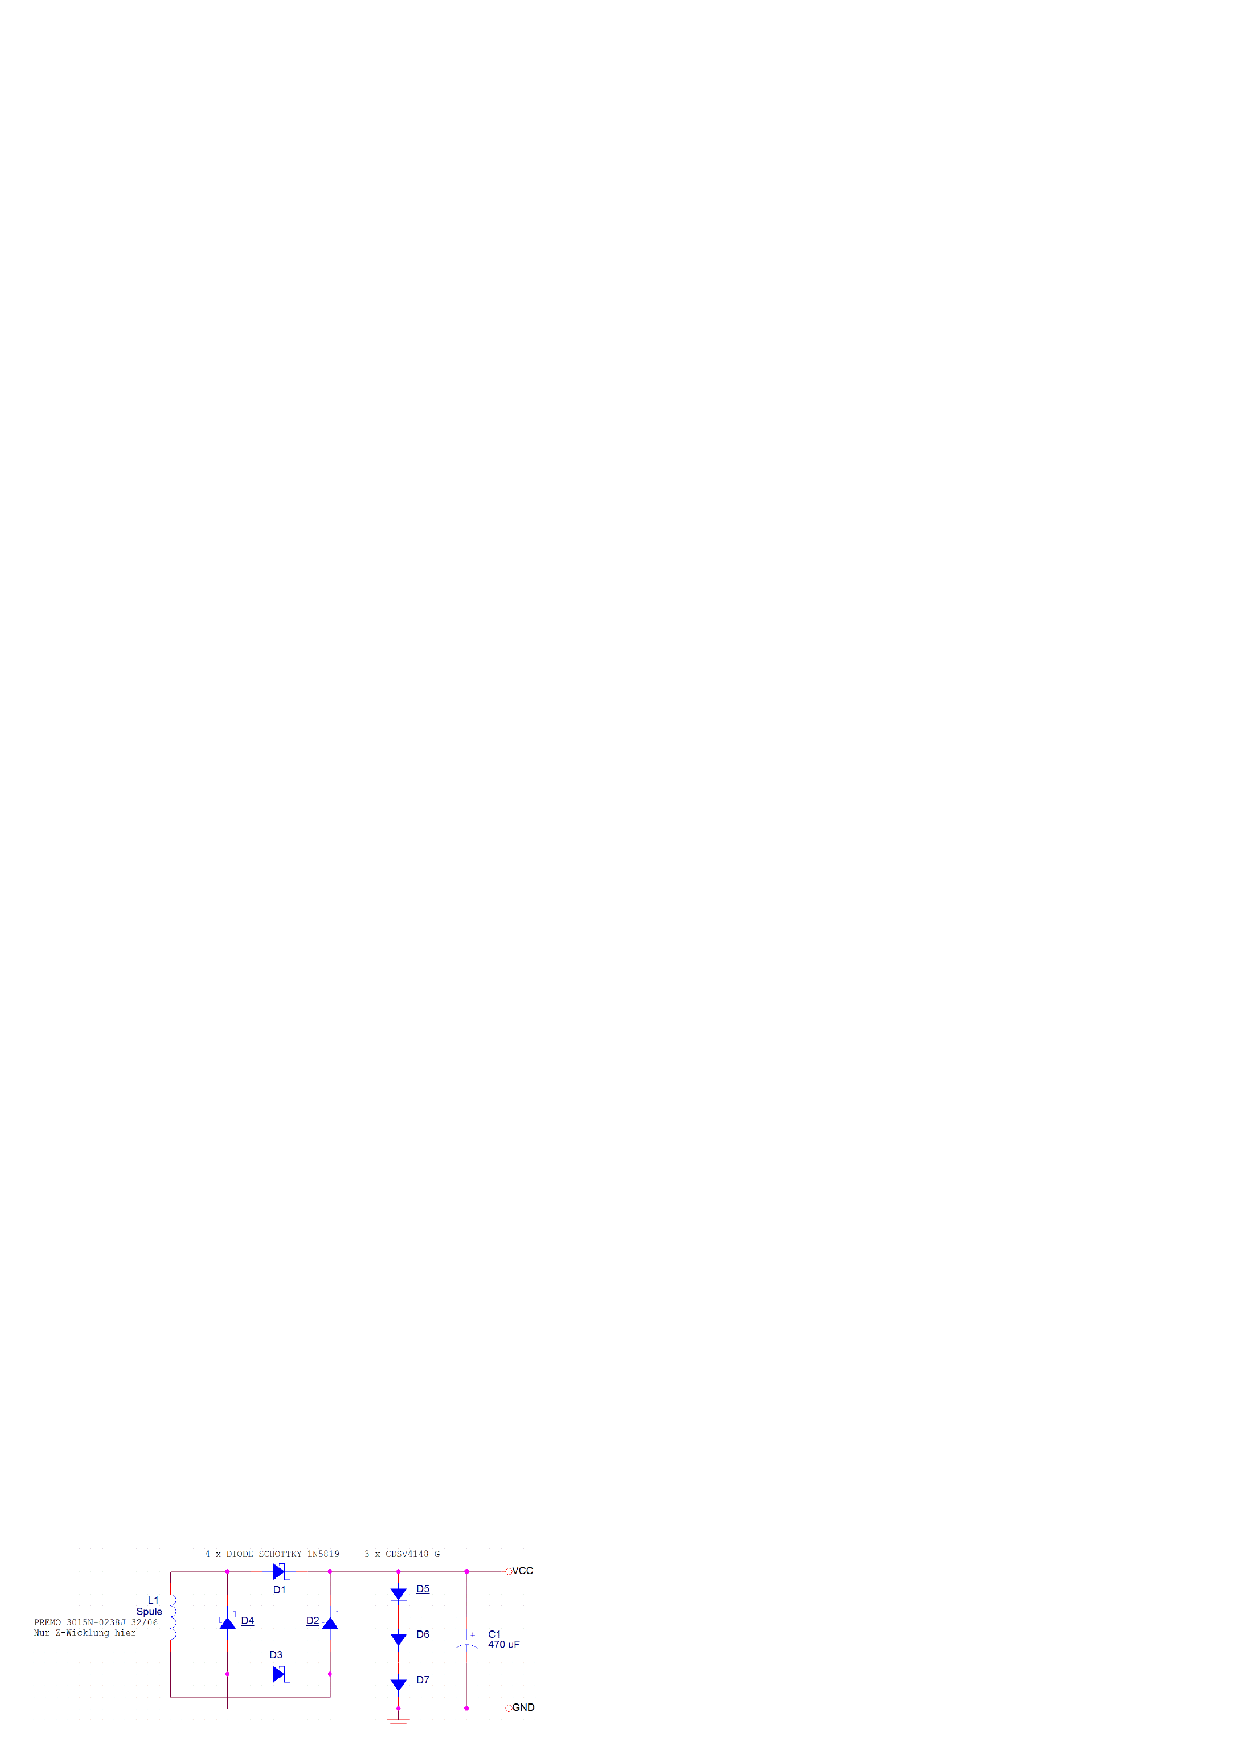
\includegraphics[width=15cm]{3Vorgehen/imag/messschaltungHarvesterschaltung.jpg}
    \caption{Messschaltung}
\end{figure}

\subsubsection*{Resultat}

Die Rippelspannung erhöht sich wie erwartet. Vpp beträgt bei 100 uF \textbf{xx} mV, bei 47 uF 28.8 mV (siehe Abbildung \ref{kond47uF}) und bei 10 uF 320 mV (Abbildung \ref{kond10uF}).
 
\begin{figure}
    \includegraphics[width=15cm]{3Vorgehen/imag/10uF.PNG}
    \caption{Rippelspannung mit 10 uF Kondensator}\label{kond10uF} 
\end{figure}

\begin{figure}
    \includegraphics[width=15cm]{3Vorgehen/imag/47uF.PNG}
    \caption{Rippelspannung mit 47 uFKondensator}\label{kond47uF} 
\end{figure}

Nach Rücksprache mit einem Entwickler des EM8500-Chips wird der zu hohe Kondensator vor dem Harvester-Eingang als Ursache vermutet. Laut Datenblatt sollte dieser 4.7 $\mu$F, damit der Booster mit eingebautem MPPT ideal regeln kann.


Aus den Beobachtungen ergaben sich folgende Aufgaben für die Entwicklung des Prototypen:

\begin{enumerate}
    \item Die Harvesterschaltung funktioniert nicht optimal. Die Auswirkung des zu hohen Kondensator vor Harvestereingang soll getestet werden
    \item Die Schaltung soll für eine Geschwindigkeit von 10 km/h ausgelegt werden
    \item Die Konfigurationen beim EM8500 sollen überarbeitet werden, sodass LTS genutzt wird
    \item Das Senden der Pakte soll der Geschwindigkeit angepasst werden
\end{enumerate}

Punkte 1 und 2 haben Auswirkung auf das Layout, Punkte 3 und 4 auf die 





%------------------------------------------------------------------------------
% 2---------------------------------------------------------------------------
%------------------------------------------------------------------------------



\section{Hardware entwickeln}

Notiz: Ziel dieses Artikels gemäss Inbetriebnahme:
- Genug Energie für BLE bei 10 km/h
\subsection{Schema}
\subsection{Bauteildefinition und Optimierung}
\subsection{Layout}

\todo{ Namensklärung: V HRV = VCC}
\todo{Messprotokolle umbenennen}


---- alter Text-----                             
Ein wichtiger Punkt der Arbeit ist die Miniaturisierung der bestehenden Hardware, das heisst der Aufbau aus der Machbarkeitsstudie soll auf eine Leiterplatte gebracht werden. Die Leiterplatte hat einige Vorgaben, welche im besten Fall alle eingehalten werden sollen.

\begin{enumerate}
    \item Die Leiterplatte soll nicht oder nur geringfügig grösser sein als das TI-SensorTag.
    
    \item Alle Netze sollen mit Testpunkten ausgestattet werden.
    
    \item Alle Anschlüsse vom TI-SensorTag sollen auf der Leiterplatte mit Testpunkten ausgestattet werden.
    
    \item Alle Testpunkte vom TI-SensorTag sollen in einem Raster von 2.54 mm angeordnet werden, damit ein Stecker kontaktiert werden kann.
    
\end{enumerate}
	


\subsection{Das Schema (oder der Stromlaufplan)}
Als erstes musste ein Schema, auch Stromlaufplan genannt, gezeichnet werden. Das Schema wurde Blockweise erfasst, als erstes wurde die Harvesterschaltung erfasst. Das Schema wurde aus der Machbarkeitsstudie entnommen. Die Funktionsweise der Harvesterschaltung kann wieder in mehrere Teile unterteilt werden.

\begin{enumerate}
    \item Die Spule: Gewinnt Energie aus dem vorbei schnellenden Magneten.
    
    \item Der Gleichrichter: Erzeugt positive Pulse aus der induzierten Spannung.
    
    \item Der Limiter: Limitiert die Spannung auf eine fixe Spannung.
    
    \item Der Ausgangskondensator: Glättet die positiven Pulse aus dem Gleichrichter.
    
\end{enumerate}

Der nächste Block ist der EM8500-Chip mit seinen Stützkondensatoren. Das Schema wurde aus dem Datenblatt entnommen. 
Die Energiespeicher, welche in dieser Arbeit mittels Elektrolytkondensatoren dargestellt werden, sind einige der wichtigsten Elemente. Die Speicherelemente werden nicht auf der Leiterplatte Platz finden, da die meisten Elektrolytkondensatoren zu hoch sind und der Platz zwischen den Leiterplatten sehr gering ist. 
Die Umlauferfassung wird mit einem Reed-Switch ermöglicht. Der Reedswitch ist einer der kleinsten Blöcke im Schema.
Der Block Interface enthält die Verbindung zum TI-SensorTag, ein Stecker realisiert dieses Interface. Der Stecker ist bereits vom TI-SensorTag vorgegeben, es handelt sich um einen Stecker, welcher sein eigenes Gegenstück darstellt. 

\subsection{Optimierung der Harvesterschaltung}

Nach dem Erfassen des Schemas wurde die Optimierung der Hardware angegangen. Die beste Optimierungsmöglichkeit und auch der kritischste Block ist die Harvesterschaltung, hier wird die Energie für die restliche Schaltung gewonnen. In mehreren Schritten wurden die einzelnen Teile der Schaltung analysiert und versucht zu optimieren.

\subsubsection{Optimierung der Spule}

Die Spule gewinnt die Energie aus dem vorbei schnellenden Magneten, hier kann die gewonnene Energie beeinflusst werden. Eine gute Spule kann mehr Energie aus dem bewegten Magneten gewinnen, wichtig ist die Induktivität L und die Fläche A, welche die Spule hat. Eine Vorgabe war dass die Spule von der Grösse nicht merklich verändert wird, ausser man würde eine kleinere Spule finden, welche mehr Energie gewinnt. Eine Spule mit ähnlicher Fläche bzw. Grösse wurde gefunden, welche eine höhere Induktivität besitzt. Die Spule von Würth Elektronik ist sehr vielversprechend, denn die gleiche Fläche mit höherer Induktivität bedeutet mehr Energiegewinn aus dem Magneten.
\todo{Hier Schlusswort von Messprotokoll einfügen}.

\subsubsection{Optimierung des Gleichrichters}

Der Gleichrichter aus dem Aufbau der Machbarkeitsstudie besteht aus vier Dioden vom Typ 1N5819, diese Dioden sind nicht für eine LowPower-Anwendung ausgelegt. Ausserdem könnte ein Gleichrichter gefunden werden, welcher in einem Gehäuse ausgeliefert wird. Wichtig ist dass der Leckstrom so gering wie möglich ist und die Schwellenspannung ebenfalls möglichst klein bleibt. 
\todo{Hier Schlusswort von Messprotokoll einfügen}.

\subsubsection{Optimierung des Limiter}

Der Limiter ist eine Spannungbegrenzung, da die nachfolgende Schaltung nicht mit einer zu hohen Spannung betrieben werden darf. Dieser Schaltungsteil ist sehr kritisch, denn er darf nicht zu viel Energie verlieren, muss aber trotzdem die Spannung immer begrenzen. Die Spannung darf einen Pegel von 2 V nicht überschreiten, da ansonsten der EM-8500-Chip droht zerstört zu werden. 
\todo{Hier Schlusswort von Messprotokoll einfügen}.

\subsubsection{Optimierung des Ausgangskondensators}

Der Ausgangskondensator muss möglichst niedrig gehalten werden, gemäss Aussage von Yves, da ansonsten der EM8500-Chip Mühe hat den Eingang zu regeln. Trotzdem darf der Ausgangskondensator nicht zu klein dimensioniert werden, da ansonsten die Rippelspannung am Ausgang der Harvestersschaltung zu hoch ist und der EM8500-Chip ebenfalls nicht mehr richtig regeln kann.
\todo{Hier Schlusswort von Messprotokoll einfügen}.


\subsection{Bauteildefinition}

Nachdem das Schema gezeichnet wurde und die Schaltung opimiert wurde, mussten die Bauteile noch definiert werden. Es mussten die Footprints, sowie die Hersteller, Herstellerbezeichnungen, Lieferant und Lieferantenartikelnummer hinterlegt werden. Einige Footprints waren bereits in den Bibliotheken vorhanden, welche wir von Lukas erhalten haben. Fehlende Footprints wurden ergänzt, wie zum Beispiel der Footprint der Spule.


\subsection{Das Layout}

\subsubsection{Positionierung}
Die Positionierung der Bauteile auf der Leiterplatte ist sehr wichtig, da hier schon unnötige Leiterbahnen gespart werden können bzw. die Länge von gewissen Leiterbahnen können extrem verkürzt werden.
Wichtig ist, dass die Stüztkondensatoren bei dem EM8500-Chip so nah wie möglich am Chip platziert werden, damit die Spannungen am Chip so konstant gehalten werden können, wie nur möglich.
Weiter sollte die Harvesterschaltung ebenfalls sehr eng beieinander platziert werden, um zu verhindern, dass durch lange Stromlaufwege bereits Leistung verloren geht. Problematisch ist, dass die Spule auf der unteren Seite der Leiterplatte platziert werden muss, somit wird die Schaltung ein auf zwei Layer aufgeteilt.
Eine grosse Herausforderung ist die Positionierung der Testpunkte, um das Interface zum TI-SensorTag zu realisieren. Dadurch wird ein grosser Platz für die korrekte Positionierung der Testpunkte eingenommen.

\subsubsection{Gestaltung der Leiterbahnen}

Wann immer möglich wurden die Leiterbahnen, welche zu der Harvesterschaltung gehören, mit 20 Mil gezogen, um eine möglichst verlustfreie Leistungsübertragung zu gewährleisten. Alle anderen nicht leistungskritischen Leiterbahnen wurden mit eine Leiterbahnbreite von 10 Mil platziert, um nicht mehr Platz in Anspruch zu nehmen als nötig.

\subsubsection{Ergebnis}

Das Ergebnis ist eine Leiterplatte, welche alle gewünschten Spezifikationen erfüllt und somit kann die Leiterplatte auch für ein Praktikum verwendet werden. Die Leiterplatte ist mit sehr vielen Testpunkten ausgestattet, sowie die Möglichkeit für Strommessungen.
\todo{Bild Neues Layout}.

% 4----------------------------------------------------------
\section{Inbetriebnahme des Prototypen}
Ziel des Kapitels: Ausmessen und sehen, dass zu wenig Energie. (Weglassen. Testteil). 2. Magnete nach 180 \% (Bild), Reellight bringt idee für 2 Magnete hintereinander, besser Spule verwenden

--- alter Text
Der entwickelte Prototyp wurde intensiv ausgemessen (siehe Messprotokolle XXXX.)  Es werden 3 Messstellen unterschieden siehe Abbildung \ref{EnergieMessungStellen}. In den folgenden Unterkapiteln werden die Resultate und die darauf folgenden Entwicklungsschritte kurz beschrieben:

\begin{figure}
  \includegraphics[width=1.0\textwidth]{3Vorgehen/imag/EnergiemessungStellen.png}\label{EnergieMessungStellen} 
  \caption{Messstellen am Prototypen}
\end{figure}

\subsection{Testen der Harvesterschaltung}

- Zu wenig Energie
- Zwei Magnete
- stärkere Spule

\subsection{Ausmessen der Energie vor und nach dem Gleichrichter}


\subsection{Energiemessungen nach dem EMBoard}



% 5---------------------------------------------------------------------------
\section{Energy Management}

Die Primäraufgabe des Energy Managements ist es, dass die zur Verfügung stehende Energie bei 10 km/h genügt, zum BLE-Pakete zu versenden. Die sekundäre Aufgabe ist es, dass man erreicht, dass sich der Long Time Storage entweder nicht lädt oder aber sich auch entlädt. Ein Laden des LTS ohne Energieabgabe ist Energieverschwendung. Die zwei gestellten Aufgaben sollen durch möglichst optimale Speichergrössen und intelligente Schwellwerte erreicht werden.

Damit man die Kondensatorenwerte berechnen kann, braucht es Energiedaten. Deshalb stehen im ersten Unterkapitel \ref{v_messungen_sensortag} Messergebnisse, danach folgt im zweiten Unterkapitel \ref{v_e_kalkulation} die Dimensionierung der Kondensatoren und dann das Berechnen der Schwellwerte in Unterkapitel \ref{v_schwellwerte}. Als letzer Punkt werden aufgrund der Ladewerte der Kondensatoren Energiezustände definiert. Dies, weil die letzte offene Aufgabe der Optimierunsliste \ref{optimierung}: Das Ersetzen des fixen Paketversendens nach 10 s dem Energiezustand angepasst werden soll. Die Vorgehensweise zur Erfüllung dieses Punktes ist im letzten Unterkapitel \ref{v_energiezustand} beschrieben. 



% x.1 ------------------------
\subsection{Energiemessungen}
\label{v_messungen_sensortag}


Die Entwicklung wird konstant begleitet durch Energiemessungen. Sei dies durch Leistungsmessungen bei der Hardware (Harvester und EM8500-Chip) oder sei dies als Energiemessung der Software (Sensortag). Für die Energiemessungen konnte der Power Analyser von Agilent Electronic N6705B mit der Serienummer MY50000795 gebraucht werden. Dieses mächtige Messgerät misst gleichzeitig Strom, Spannung und somit die Leistung im Zeitverlauf. Mühsame Annäherungen aus eigenen KO-Messungen sind somit nicht mehr notwendig.
In diesem Unterkapitel werden die Resultate vielre Messungen in ihrer zeitlichen Reihenfolge zusammengefasst. Die Detailaufnahmen zu allen Messungen finden sich in der CD im Ordner Messungen in der Datei Energiemessungen.pdf. 



\subsubsection{Erste Energiemessungen}
\label{erst_EMessungen}

\todo{Graphik kommt nicht heraus}

\begin{figure}[ht]
    \includegraphics[scale=1]{3Vorgehen/imag/v0Send33uJ.png} 
    \caption{Minimalster Energieverbrauch: 3 BLE Pakte über Advertising Mode senden}
    \label{BLE_send}
\end{figure}

Um einen Anhaltspunkt über den Energieverbrauch des Sensortags zu erhalten, wurde 3 BLE-Pakete im Advertsing Mode per Knopfdruck gesendet (siehe Abbildung \ref{BLE_send}). Dies entspricht der Messung zur Sensortagversion V0. Nach der Weiterentwicklung des Programms, folgte die Messung V1, in der zusätzlich die GPIO ausgelesen werden. Dies ist für das Einlesen der Reed Switch-Impulse unumgänglich und für das Einlesen der Energy States vom 8500 sinnvoll. Die Version V2, erster Versuch mehr Sleep-Time einzubauen, scheiterete am Zusammenspiel des Timings der Radio- und GPIO-Interrupts. Das Neuaufsetzen des Programms half, sodass die Version V3 power-optimiert Geschwindigkeitspakete sendet. Die untenstehende Tabell stellt die ersten Energieresultate dar. Unterschieden wird zwischen dem Energieverbrauch für die Initialisierung und der Energie zum Senden von 3 BLE Paketen. Die Diskussion über Energieoptimierungen und die Deutung der Resultate finden sich in den Sitzungsprotokollen vom xxxxx - xxxx. Die Energiemessungen im Detail sind abgelegt auf der CD gemäss der Auflistung im Anhang xxxx.
\todo{Sitzungsprotokolle Datum einsezten, Anhanhgsbezeichnung}

\subsubsection*{Messresultate nach Sensortag-Versionen}
\begin{tabbing}
    Version   \quad\= Datum    \quad\= Was................................................... \quad\= Energie Init    \quad\=  Energie Senden \\[0.8ex]
    V0        \> 10.3.16  \> Nur BLE Paket      \> unbekannt            \> 33 $\mu$J \\
    V1        \> 16.3.16  \> mit Geschwindigkeit      \> 87 $\mu$J            \> 32 $\mu$J \\
    V3        \> 22.4.16   \> Schlafmodus optimiert     \> 40 $\mu$J            \> 29 $\mu$J \\
    V4        \> 03.6.16    \> 3 Sensore, kein Schlafmodus optimiert     \> 77 $\mu$J            \> 43 $\mu$J \\
\end{tabbing}

Bei den ersten drei Messungen werden die Sensoren noch nicht ausgelesen. Es zeigt sich, dass das Auslesen der Sensoren über I2C und das Warten, bis dass die Sensoren aufgestartet sind, viel mehr Energie verbraucht, als erwartet. Der Energieverbrauch des Auslesens nur eines Sensors (erste Priorität hat laut Aufgabenstellung der Drucksensor) ist ohne Optimierungsmassnahmen so gross, dass kein Senden der Daten mehr möglich ist. Die Speisung der Applikation bricht sofort zusammen (siehe Abbildung \ref{i2c_problem}).
\todo{warum ht sich BLE verschlechtert?}

\begin{figure}[ht]
    \includegraphics[scale=1]{3Vorgehen/imag/pic4VSUPbrichtEin.PNG} 
    \caption{Auslesen der Sensoren reisst Energie zusammen}
    \label{i2c_problem}
\end{figure}

\todo{Bild erscheint nicht}

Aus diesen Grund wurde die Power-Optimierung innerhalb des Programms zur zentralen Herausforderung in dieser Arbeit. Details darüber sind im nächsten Unterkapitel \ref{powerOptimierung} Power Management zusammengefasst. Hier die Auflistung der Energiewerte von Version V4. Bei dieser Version werden die Sensoren ausgelesen und dazwischen geht das Sensortag in den Schlafmodus, damit sich der Primärkondensator wieder laden kann. Erst nachdem alle Sensoren ausgelesen sind, wird das BLE-Paket versendet.



\subsubsection{Sensortag}
\label{energie senosortag} 

Der Energieverbrauch des Sensortags wird 4-mal gemessen. Einmal mit der Minimalversion: Nur Pakete mit Geschwindigkeitsdaten senden. Dann diese Version mit den drei Sensoren, die einer nach dem anderen ausgelesen werden. Weil dazwischen geschlafen wird, damit das System wieder genug Energie gespeichert hat, dauert diese Version xxx s \todo{Zeit eintragen}. Von jedem Sensor wird der eigene Energieverbrauch ermittelt, um einen Vergleich unter ihnen herstellen zu können.

\paragraph{Nur Geschwindigkeit: Simple Harvester}

\todo{Energiemesssung OHNE Sensoren. Aber mit Warten}

%\begin{figure}
%  \includegraphics[width=1.0\textwidth]{idle.png}
%  \caption{Energieverbrauch nur Geschwindigkeit Senden V4}
%  \label{messung_v}
%\end{figure}



\paragraph{Energieverbrauch Drucksensor}

Auf dem Sensortag wird der Drucksensor BMP 208 von Bosch Sensortec verwendet. Der Druckwert wird über I2C ausgelesen. Hier die Energiemessung des Sensors, ausgelesen mit der Sensortag Version 4, am 3. Juni 2016.

\begin{figure}[ht]
  \includegraphics[width=1.0\textwidth]{3Vorgehen/imag/Drucksensor.png}
  \caption{Energieverbrauch des Drucksensors BMP 280}
  \label{energie_drucksensor}
\end{figure}

Das Auslesen des Drucksensors verbraucht 5.753 $\mu$J.

\paragraph{Energieverbrauch Temperatursensor}

\todo{tempsensor daten}
Der Temperatursensor xxx der Marke yyy verbraucht fürs Auslesen der Daten, ohne Energieoptimierung, 10.635 $\mu$J.

\begin{figure}[ht]
  \includegraphics[width=1.0\textwidth]{3Vorgehen/imag/tempSensor.png}
  \caption{Energiemessung Temperatursensor auf Sensortag}
  \label{energie_tempsensor}
\end{figure}


\paragraph{Energieverbrauch Feuchtigkeitssensor}

Der Feuchtigkeitssensor verbraucht 6.358 $\mu$J, siehe Abbildung \ref{energie_humidity}.

\begin{figure}
  \includegraphics[width=1.0\textwidth]{3Vorgehen/imag/Humidity.png}
  \caption{Energieverbrauch Feuchtigkeitssensor}
  \label{energie_humidity}
\end{figure}




% x.2 ---------------------------------
\subsection{Energiekalkulation}
\label{v_e_kalkulation}

Der Energieverbrauch hängt von der Anzahl ausgelesener Sensoren ab (siehe \ref{v_messungen_sensortag}). Für die Bestückung der Kondensatoren wird vom schlechtesten  Fall, einer Geschwindigkeit von 10 km/h ausgegangen. Die Grundlagen zur Energiekalkulation $\bar{E_{HRV}} \ge \bar{E_{BLE}} $ sind im Theorieteil \ref{th_energiebilanz} abgebildet. Hier werden die Kondensatoren berechnet.

\todo{Gleichungen zusammen. Berechnung konkret}
\begin{equation}
  C_{STS}= \frac{ E_{Applikation}}{(V_{STS\_HIGH} )^2 - (V_{STS\_LOW} )^2}
\end{equation}

\begin{equation}
  C_{STS}= \frac{ E_{Applikation}}{(3.6 V )^2 - (2.1 V)^2}
\end{equation}

\begin{equation}
  C_{STS}= \frac{ E_{Applikation}}{(3.6 V )^2 - (2.1 V)^2}
\end{equation}

\begin{equation}
  C_{STS}= \frac{ E_{Applikation}}{(3.6 V )^2 - (2.1 V)^2}
\end{equation}


\todo{Abschlusstext. Übergang}

\subsubsection{MPP einstellen}

\todo{Messprotokolle eintrage}

Das Ziel der Entwicklung ist, dass bei einer Geschwindigkeit von 10 km/h genug Enerige zum Senden eines BLE-Pakets zur Verfügung steht. Während der Entwicklung des Harvesters wurde die Leistungskurve öfters aufgenommen (siehe Anhang \ref{uebersicht_messprotokolle}, xxx,yyy, zz). Wie im Theorieteil erklärt \ref{harv_diff} unterscheidet sich das Leistungsmaximum nach Geschwindigkeit. Weil das Ziel ein funktionstüchtiger Prototyp bei 10 km/h ist, bezieht sich das Einstellen nur auf diese Wert.  

 
\subsubsection*{MPP-Ratio bei 10 km/h gemäss Messprotokollen}
\begin{tabbing}
    Datum       \quad\= Leistungmaximum    \quad\= MPP-Ratio\\[0.8ex]
    30. März    \> 12 $\mu$W        \> 43.23\thinspace\% \\
    xx          \> xx $\mu$W        \> xx\thinspace\%\\
    resultat    \> 21.87  $\mu$W    \> 24.87\thinspace\%\\
\end{tabbing}\todo{Werte}

Es zeigt sich, dass das Leistungsmaximum unterhalb von 50\thinspace\% liegt. Bedauerlich ist, dass durch die Energieoptimierung sich die Stelle des Leistungsmaximums Richtung Leerlauf verschiebt. In der Umsetzung mit dem EM8500-Chip ergibt sich das Problem, dass nur Konfigurationen von MPPT-Ratios von 50 - 80\thinspace\% erlaubt sind (siehe Tabelle unten).  Die Einstellungen der tieferen MPP-Ratio sind zudem gröber. Dies, weil der EM8500-Chip für Harvester vom Typ TEG (mit einem MPP konstant bei 50\thinspace\%) und Solarzelle konzipiert ist und die MPPT-Ratio für diese zwei Anwendungen genau in diesem Range liegen. In unserem Fall ist dieser vorgegebene Range nicht ideal. Da beim energiekritischen Zustand bei 10 km/h die Ratio deutlich unter 50\thinspace\%. Die Vorgänger wählten in ihren Einstellungen eine MPPT-Ratio von 88\thinspace\%. Die Vermutung liegt nahe, dass keine Leistungskurve des Harvesters im Voraus aufgenommen wurde.


\subsubsection*{MPPT-Ratio Einstellungen EM8500}
\begin{tabbing}
    Registerwert   \quad\= MPPT-Ratio    \\[0.8ex]
    0x00           \> 50\thinspace\% \\
    0x01           \> 60\thinspace\%\\
    0x02           \> 67\thinspace\%\\
    0x03           \> 71\thinspace\%\\
    0x04           \> 75\thinspace\%\\
    0x05           \> 78\thinspace\%\\
    0x06           \> 80\thinspace\% \\
    0x07           \> 82\thinspace\%\\
    0x08           \> 83\thinspace\%\\
    0x09           \> 85\thinspace\%\\
    0x0A           \> 86\thinspace\% \\
    0x0B           \> 87\thinspace\%\\
    0x0C           \> 88\thinspace\%\\
\end{tabbing}

\todo{Sitzungsprotokoll Datum}
Im ersten Versucht wird das Register auf das Minimum (50\thinspace\%) eingestellt (siehe Sitzungsprotokoll YYYY). Die Messung ergab, dass bei 10 km/h das EM-Board nicht gespiesen wird. So luden sich weder der STS noch der LTS auf. Der Grund ist, dass der optimale Leistungsbezug bei 50\thinspace\% liegt, das Leistungsmaximum aber später. So entstand beim Regeln auf den optimalen Leistungsbezug der Umstand, dass dort nur 0.2 V produziert werden. Dieser Spannungswert ist zu tief, der EM-Chip beginnt nicht zu arbeiten. Betreibt man den Harvester nicht am optimalen Punkt, sondern bei einer MPPT-Ratio von 60\thinspace\%, so wird eine Eingangsspannung von 0.3 V produziert und EM8500 beginnt zu arbeiten.




% x.3 -------------------------------------
\subsection{Einstellen der Schwellwerte}
\label{v_schwellwerte}

Das Konzept der Schwellwerte von VSTS und VLTS sind im Theorieteil bei der Erklärung des Speicherkonzepts des EM8500-Chips im Unterkapitel \ref{speicher_konzept} beschrieben. Das Ziel ist, dass bei 10 km/h sich LTS entlädt. Die Berechnung der Schwellwerte stammt aus dem Theorieteil \ref{th_energiebilanz}.




Aus der Vorgängerarbeit sind in der Tabelle unten notierte Konfigurationswerte überliefert. Bei der Inbetriebnahme fiel der hohe Schwellwert von v\_bat\_min\_hi\_dis auf (3.6 V), ab der erst die Applikation gespiesen wird. Den hohen Wert beruht auf dem Versuch, möglichst viel Energie vor dem Datensenden zu sammeln. Ein hoher Schnellwert verzögert die Zeit, bis zum ersten Datensenden.

\subsubsection*{Konfiguration Vorgängermodell}
\begin{tabbing}
    Register .............\quad\= Wert \\[0.8ex]
    v\_bat\_max\_hi       \> 4.2 V \\
    v\_bat\_max\_lo       \> 4.1 V \\
    v\_bat\_min\_hi\_dis  \> 3.6 V \\
    v\_bat\_min\_hi\_con  \> 2.1 V \\
    v\_bat\_min\_lo       \> 1.8 V \\
    v\_appl\_max\_hi      \> 3.8 V \\\
    v\_appl\_max\_lo      \> 3.7 V \\ 
    mppt\_ratio            \> 88\thinspace\% \\
\end{tabbing}

Nach der Energiemessungen der Version V3 des Sensortags (siehe \ref{erst_EMessungen}), in dem die Geschwindigkeit per BLE gesendet werden kann, entstanden folgende Schwellwerte:

\subsubsection*{Erste Konfiguration aufgrund Geschwindigkeitsmessung}
\begin{tabbing}
    Register .............\quad\= Wert \\[0.8ex]
    v\_bat\_max\_hi       \> 4.8 V \\
    v\_bat\_max\_lo       \> 4.7 V \\
    v\_bat\_min\_hi\_dis  \> 2.6 V (siehe Berechnungen unten)\\
    v\_bat\_min\_hi\_con  \> 2.1 V \\
    v\_bat\_min\_lo       \> 2.0 V (vorgegeben von Sensortag)\\
    v\_appl\_max\_hi      \> 3.8 V \\\
    v\_appl\_max\_lo      \> 3.7 V \\ 
    mppt\_ratio            \> 50\thinspace\% (aus MPP-Kurve Harvester)\\
\end{tabbing}

Die Grundlage bildete die Gleichung  $E_{Applikation}= E_{STS\_HIGH} - E_{STS\_LOW}$, wobei  $E_{Applikation}$ aus der Messung von V3 mit total 93.2 $\mu$J für die Initialisierung und das Senden der Daten gebraucht werden, und $V_SUP$ durch das Sensortag mit 2.0 vorgegeben ist. Laut Datenblatt des EM8500 (\cite{datasheet_EM85}, S. 9, Abschnitt Operating Conditions ) soll STS zwischen 10 - 100 $\mu$F gross sein. Typisch ist 47 $\mu$F. Um auf der sicheren Seite zu sein, denn der Harvester gibt zu diesem Zeitpunkt noch nicht genug Energie ab, wurde als Berechnungsgrundlage C\_{STS} von 100 $\mu$F genommen.  So ergab sich folgender minimaler oberere Schwellwert:

\begin{equation}
(v\_bat\_min\_low) ^2  =  \frac{2\, \times \, E_{Applikation}}{C_{STS}} + (V_{STS\_LOW})^2
\end{equation}

\begin{equation}
(v\_bat\_min\_low) ^2  =  \frac{2\, \times \, 93.2, \mu J}{100 \,\mu F} + (2.0)^2
\end{equation}

\begin{equation}
v\_bat\_min\_low  =  \sqrt{\frac{186.4}{100 } + 4} = \sqrt{5.864} = 2.42 V
\end{equation}

Alternativ kann man den laut Datenblatt vorgeschlagenen Kondensatorenwert von  47 $\mu$F. Dann ergibt sich als oberer Schwellwert  $v\_bat\_min\_low  =  \sqrt{\frac{186.4}{47 } + 4} = \sqrt{7.97} = 2.82, V$. Als erstes wird der Schwellwert auf 2.6 V gesetzt. Wichtigster Wert in der Konfiguration ist jedoch der korrekte MPPT-Wert. Er wird auf das Minimum (50\thinspace\%) gesetzt. Das Maximum des Ladezustands  wird auf den maximal erlaubten Wert gesetzt: v\_bat\_max  = 4.8 V bzw. 4.7 V. Denn solang Energie geerntet werden kann, soll sie gespeichert werden. v\_appl\_max spielt in unserer Anwendung keine wichtige Rolle. Der Wert wird von den Vorgängern übernommen.

\todo{Messprotokoll und Sitzungsprotokoll einfügen}
Das Zusammensetzen der Last (Sensortag) mit der konfigurierten Hardware erstaunte (siehe Messprotokoll xxx und Sitzungsprotokoll yyy). Ab 25 km/h funktionierte die Schaltung gut. Doch darunter reagiert der EM8500-Chip nicht. Weder STS noch LTS konnten sich laden. Nachmessungen am Eingang vom EM8500-Chip ergaben, dass bei  10 km/h und einer MPPT-Ratio von 50\thinspace\% eine Spannung von 0.2 V anliegt. Diese ist zu tief, um den Booster zu starten. Erst bei höherer Geschwindigkeit wird eine Eingangsspannung von mehr als 0.3 V erreicht, und das System beginnt zu funktionieren. Aus diesem Grund wird die MPPT-Ratio zukünftig auf den zweittiefsten Wert (60 \thinspace\%) eingestellt. 

Ein unerwartetes Verhalten zeigt sich bei der Implementation des Auslesen des ersten Sensors, der Drucksensor. Der BLE-Sniffer empfängt die Druckdaten korrekt, doch beim Anschliessen des Sensortags an den Harvester, riss die Spannung sofort zusammen. Innert kürzester Zeit haben sich entlädt sich der STS wie parallel zu ihm der LTS und unterschreitet der STS den Schwellwert von V\_SUP von 2 V, so stellt die Speisung der Applikation ab (siehe Abbildung \ref{i2c_problem} im Unterkapitel \ref{erst_EMessungen}). Das Ausmessen des Energieverbrauchs bringt Klarheit: Die I2C-Kommunikation und das Aufstarten des Sensors brauchen xxx-mal mehr Energie, als das Berechnen der Geschwindigkeit aus den Reed-Switch Impulsen (siehe Abbidlung yyy im Resultat-Teil).
\todo{link zu Abbildung im Resultat Teil. Faktor ausrechnen}

Durch den deutlich höheren Energieverbrauch, wird eine Power-Optimierung im Softwareteil notwendig. Es zwingt aber auch, den Schwellwert von v\_bat\_min\_hi\_dis  wieder zu erhöhen. Die finale Konfiguration ist im Resultate-Teil abgebildet.


% x.4 -----------------------------------------
\subsection{Energiezustand des Systems}
\label{v_energiezustand}

Die letzte der vier Aufgaben aus der Optimierungsliste nach der Inbetriebnahme (siehe Unterkapitel \ref{optimierung}) ist das variable Anpassen des BLE-Paketsendens aufgrund des Energiezustandes. Im ersten Unterkapitel \ref{def_zustaende} wird das Einteilen des Systems in Energiezustände beschrieben, danach die Umsetzung in Software im Prototyp angewendet wurde. 

\subsubsection{Definition von Energiezuständen}
\label{def_zustaende} 

\
Da die produzierter Energie von der Fahrgeschwindigkeit abhängt, wird das Energiesystem in drei Zustände eingeteilt, die von der Geschwindigkeit abhängen:

\subsubsection*{Energiezustände aufgrund der Geschwindigkeit}
\begin{tabbing}
   0 - 15 km/h      \quad\= LOW\_ENERGY   \\[0.8ex]
   15 - 25 km/h      \> MIDDLE\_ENERGY \\
   $>$ als 25 km/h   \> HIGH\_ENERGY\\
    
\end{tabbing}

Was in den eingelnen Energiezuständen gemacht wird:

Bild

\subsubsection*{Energiezustände: Umsetzung in Software}






 4---------------------------------------------------------------------------
\section{Power Management}
\label{powerOptimierung}

Aufgrund von Messungen -> Codeoptimierung


%... noch zu schreiben ....
%Üblicherweise wird das RTOS-Betriebssystem von TI für Low Power Applikationen benutzt. 


%(Die Low-Power Programmbeispiele von TI basieren auf RTOS, ebenso die Dokumentation zu Low Power Applikationen, was zu viel Energie verbraucht (korrekt, wie belegen?). )


%Problem: So gehört zu jedem Aufwecken einer Peripherie, der Parallele Schlafmodus, bis dass die Peripherie gestartet ist. (Dies gilt auch für die Sensoren.) Zu lange warten: braucht Energie.
%
%Sleep konkret: Power Banks abschalten:\\
%Power Domains zeigen
%
%Schwierigkeit Interrupt and Events !!
%
%Bild: Energie-Langzeitmessung BLE versenden\\
%Beschriften mit aktiv und standby modus
%
%
%Gearbeitet wird mit einem Cortex M3 von TI.\\ 
%Grundsätzlich basieren die Bsp. auf RTOS. Wenige für PowerManagement. Das Powermanagement ohne Betriessystem. Wir verwenden dies, weil (gemäss Erfahrungswerte Praxis) mit Betriebsystem mehr Energie braucht).


\begin{figure}
  \includegraphics[width=1.0\textwidth]{../ressources/SimpleLink/V0Sendeablauf.png}
  \caption{Prozessablauf V0}
\end{figure}




% 5 ---------------------------------------------------------------------------
\section{Applikationsentwicklung}

\subsection{Aufbau der App}

\subsubsection{BLE empfangen und filtern}

\subsection{Grundeinstellungen}

\subsection{Tachometer einbauen}

\subsection{Modularer Aufbau}

Die Applikationsentwicklung basiet auf einer modularen Struktur.  Dadurch wird eine Weiterentwicklung der Applikation ohne Probleme möglich. Ebenfalls wurde beachtet, dass die Applikation sogar in andere Sprachen übersetzt werden können muss, dafür wurden alle Texte, die ersichtlich sind in einem File aufgenommen und können zentral abgeändert werden, ohne einen Eingriff in den aktuellen Code.


Mit Android Version xx.

--- alter Text --- 

\subsection{Aufbau der App}

Welche Aktion zu welchem Display gehört (Überblick Gesamtsystem)


\subsection{Implementierte Aktionen}
Geräteauswahl
Kalibrierung
Geschwindigkeitsberechnung
Sensordaten ausgeben (was mit welcher Genauigkeit)

\subsection{BLE Empfangen}

Aufbau des Datenpakets: 
LEN, UUID, ...






